	
	\subsection*{1.}
	
	Recopier sur la copie et compléter l’arbre pondéré ci-dessous :
	
\begin{center}
	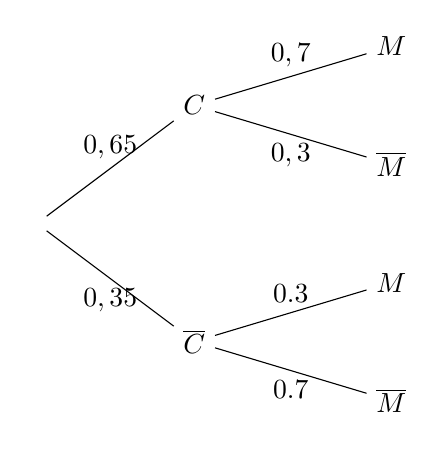
\begin{tikzpicture}
		[level 1/.style={level distance=2cm,
			sibling distance=3cm},
		level 2/.style={level distance=2.5cm,
			sibling distance=1.5cm}]
		\node {} [grow'=right]
		child {node {$C$}
			child {node {$M$}
				edge from parent node[above] {$0,7$}
			}
			child {node {$\overline M$}
				edge from parent node[below] {$0,3$}
			}
			edge from parent node[above] {$0,65$}
		}
		child {node {$\overline C$}
			child {node {$M$}
				edge from parent node[above] {$0.3$}
			}
			child {node {$\overline M$}
				edge from parent node[below] {$0.7$}
			}
			edge from parent node[below] {$0,35$}
		}
		;
	\end{tikzpicture}
\end{center}
	
	\subsection*{2.}
	
	\[
	P(C \cap M) = P(C) \times P_C(M) = 0,65 \times 0,7 = 0,455.
	\]
	
	\subsection*{3.}
	
	On a de même \(P(\overline{C} \cap M) = P(\overline{C}) \times P_{\overline{C}}(M) = 0,35 \times 0,3 = 0,105\).
	
	D’après la loi des probabilités totales :
	\[
	P(M) = P(C \cap M) + P(\overline{C} \cap M) = 0,455 + 0,105 = 0,56.
	\]
	
	\subsection*{4.}
	
	On doit calculer \(P_M(C)\) :
	\[
	P_M(C) = \dfrac{P(M \cap C)}{P(M)} = \dfrac{P(C \cap M)}{P(M)} = \dfrac{0,455}{0,56} = 0,8125.
	\]
	
	\subsection*{5.}
	
	Une semaine de pension complète coûte 800 €.
	
	Une semaine de demi-pension coûte 650 €.
	
	L’option « ménage » coûte 50 €.
	
	On ne peut arriver à un montant de 850 € que si on prend la pension complète et l’option « ménage ». On a donc :
	\[
	P(X = 850) = P(C \cap M) = 0,455.
	\]
	
